
 
\documentclass{article}
\usepackage{indentfirst} % indentation
\usepackage[margin = 2cm,includefoot]{geometry}
\usepackage{graphicx}  %import images
\usepackage{float} %control float positions


\usepackage[hidelinks]{hyperref}  % hyper links

\usepackage{mhchem}  % chemistry equations

\usepackage{xfrac}  % slanted fraction



%___________footer and header _______________
%\usepackage{fancyhdr}
%\pagestyle{fancy}
%\fancyhead{}
%\fancyfoot{}
%\fancyfoot[R]{\thepage}
%\renewcommand{\headrulewidth}{1pt}


\begin{document}
\begin{titlepage}
	\begin{center}
		\line(1,0){400}\\
		[3mm]
		\huge{\bfseries Report1}\\
		[3mm]
		\textsc{\LARGE paper name }\\
		[10cm]
			
	\end{center}
     
     \begin{flushright}
     \LARGE{Jinxi Liu}
     \end{flushright}
     
\end{titlepage}
	
\tableofcontents
\cleardoublepage

\listoffigures
\addcontentsline{toc}{section}{\numberline{}List of Figures}
\cleardoublepage

\listoftables
\addcontentsline{toc}{section}{\numberline{}List of Tables}
\cleardoublepage

\section{Introduction}\label{section1}
\par
This article discussed the false discovery rate in the settings where the ordered of hypothesis was prespecified. 


Paragraph2
\newpage
\section{Section2}

% table and figures
\subsection{Subsection1}

\begin{figure}[H]
		
	 \centering
	 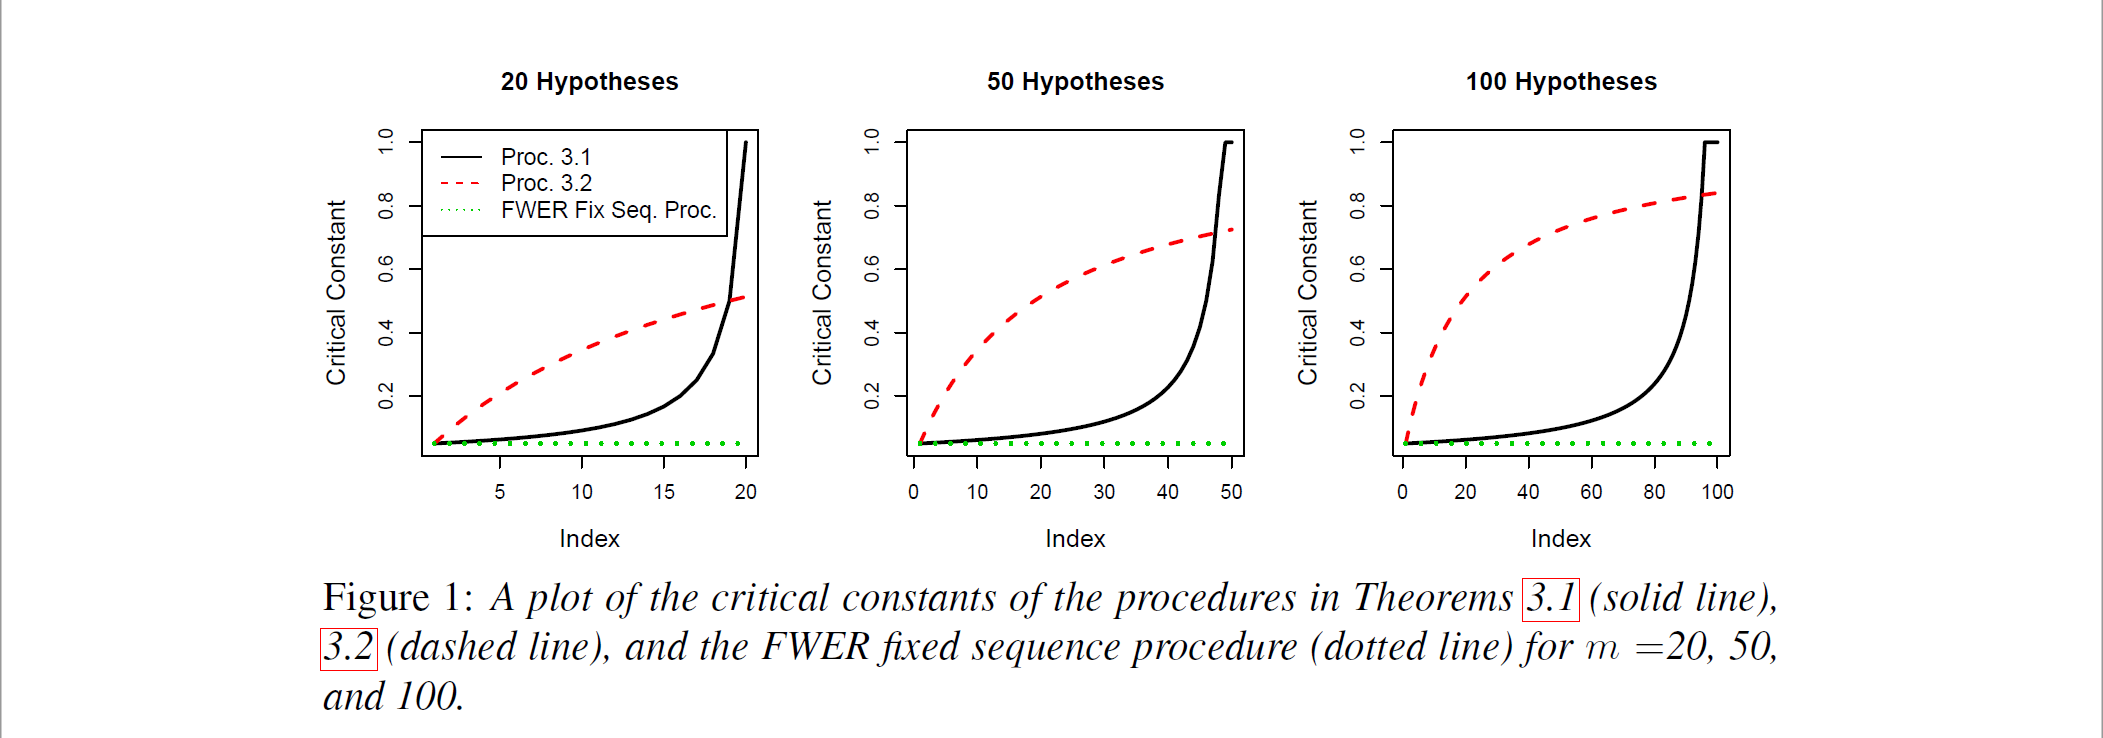
\includegraphics[height=3in]{C:/Users/jeffl/desktop/test}
	 \caption[Optional caption]{Real caption to display}
	 \label{fig1}
	 
\end{figure}

Figure \ref{fig1} shows...\\

\vspace{2cm}

\begin{table}[H]
	
	\centering
	\caption{Real caption to display}
	\label{tab1}
	
	\begin{tabular}{c c c c}
		\hline
		\bfseries{Patid} & \bfseries{Visit} & \bfseries{Treatment} & \bfseries{Weight}\\ \hline
		11011 & BAS   & Placebo & 100 \\
		11012 & BAS & Metformin & 120\\
		\hline
	\end{tabular}
	
\end{table}
Table \ref{tab1} shows...


% lists
\renewcommand{\labelitemi}{$\bullet$}
\renewcommand{\labelitemii}{$\diamond$}
\renewcommand{\labelitemiii}{$\circ$}

\subsection{Subsection2}
This is a list:
\begin{itemize}
	\item This is the first item
	\begin{itemize}
		\item sub item
		\item[title] second sub
	\end{itemize}
	\item looooooooooooooooooooooooooooooooooooooooooooooooooooooooooong item.
	\item item 3!
	  \begin{enumerate}
	  	\item list with numbers
	  \end{enumerate}
\end{itemize}

\subsection{Subsection3}
Math:\\
For example: $E=mc^2$ or $$a = b + c $$ 
$$\frac{\bar{x}}{2\hat{x}}\frac{d\sigma^2}{d\sigma}$$

CE:
\ce{CH_4(g) -> CO_2(g)}

$$d_(i) = \sfrac{1}{2}\cdot t ^2 $$

Brackets:\\
$$\left( \frac{1}{2} \right) = 0.5 $$
$$ { \frac{1}{2}} = 0.5 $$
$$ \left|-7 \right| = 7 $$
$$ x^{2^3} $$
$$ \sqrt{4} =2 $$
$$ \sqrt{4} \neq 3 $$
$$ \pi \approx 3 $$ 
$$ x \times 2 $$
--------------------------------------------
\begin{eqnarray*}
	\left( \frac{1}{2} \right) &=& 0.5 \\
	 { \frac{1}{2}} &=& 0.5 \\
	\left|-7 \right| &=&  7 \\
	 x^{2^3} \\
	\sqrt{4} =2 \\
	\sqrt{4} \neq 3 \\
	 \pi \approx 3 \\
	x \times 2 
\end{eqnarray*}


————————————————————————————————————
\begin{equation}\label{refeqn1}
\left( \frac{1}{2} \right) = 0.5 
\end{equation}

Test the equation reference: \ref{refeqn1}.

\cleardoublepage

\bibliographystyle{IEEEtran}
\bibliography{}	 
\end{document}